\documentclass{article}
\usepackage{graphicx} % Required for inserting images
\usepackage{amsfonts,fullpage}
 \usepackage{amssymb}
\usepackage{amsmath}
\usepackage{graphicx}
\usepackage{tikz}
\usetikzlibrary{arrows.meta,automata,positioning}
\usepackage{algorithm}% http://ctan.org/pkg/algorithm
\usepackage{algpseudocode}
\usepackage{float}
 
\usepackage{amsthm}
\newtheorem{theorem}{Theorem}
\newtheorem{definition}{\color{bluem}Definition}
\newtheorem{lemma}[theorem]{Lemma}
\definecolor{bluem}{rgb}{0.0, 0.5, 0.69}

\title{\textit{MP-Allop-2} and  \textit{Sub-Network Redirect and Preserve Ploidy (SRPP)}: A Novel Network Move for Inference of Polyploid and Allopolyploid Networks}
\author{Mark Kessler, Zhi Yan, Dr. Luay Nakhleh, Dr. Huw Ogilvie}
\date{March 2024}

\begin{document}

\maketitle

\section{Abstract}
Polyploidy has been shown to be prevalent not only in plants but also in other groups of eukaryotic species, but 
most work done thus far on phylogenetic network inference assumes standard diploid hybridization. 
These inference methods have been applied, with varying degrees of success, to data sets with allo/autopolyploid species, 
even though polyploidy violates some certain mathematical assumptions underlying these methods. 
  
In this paper, we introduce an improved method of the previously implemented InferNetwork-MP-Allop in PhyloNet (Yan et al.) for inferring parsimonious phylogenetic networks on data that include polyploid 
and autopolyploid species. Taking gene tree topologies and a taxon mapping as input, the method will infer a phylogenetic network that minimizes deep coalescences while accounting for polyploidy, incomplete sampling, and ILS.
  
This new method employs a single network move (rather than 6 independent moves) that combines aspects of SPR with the ability to only propose networks that
satisfy the ploidyness of the taxa, which has the effect of reducing time spent proposing networks that would simply be rejected on the basis of incorrect topology.
We will show a drastic decrease in runtime, as well as a empirical data that shows that this one move is sufficient to explore the entire network space.

Also, this method will be more flexible and robust than prior iterations. For example, AlloppNET (2013) can only infer networks with exactly 2 diploid species and 1 tetraploid clade-- it is also a bayesian method that is extremely slow when compared to parsimony. InferNetwork-MP-Allop (2022), one such parsimony method, is 100x faster than AlloppNET. However it uses many network moves, only supports
fixed polyploid clade membership, and does not support autopolyploid "bubbles". Our improved method, MP-Allop-2, is over 100x faster than InferNetwork-MP-Allop and 10000x faster than AloppNET, while also supporting autopolyploidy and variable clade membership.

\section{Polyploidy and Allopolyploidy}
In phylogenetics, allopolyploid and polyploid species play significant roles in understanding evolutionary relationships and genetic diversity. Allopolyploids arise from the hybridization of two distinct species, resulting in a genome containing sets of chromosomes from each parental species. These hybrids often exhibit increased genetic variation, potentially leading to enhanced adaptability and speciation. On the other hand, polyploid species possess multiple sets of chromosomes within their genomes, which can arise through various mechanisms such as genome duplication events.

In addition to their importance in understanding evolutionary relationships and genetic diversity, polyploid species also present unique challenges and opportunities in network inference analyses. Previous phylogenetic network methods have struggled  to accurately and fully represent the complex evolutionary histories and genetic interactions within polyploid genomes in a time efficient manner.


\paragraph{\color{bluem}A New Method is Needed}

While InferNetwork-MP-Allop solved many of the performance and inflexibility issues present in AlloppNet via switching over to the parsimony approach of minimizing deep coalescences in a MUL (MULtilabeled Species Tree) tree, there are two key ways in which it can be made to be more adaptable to more biological scenarios.

First, InferNetwork-MP-Allop does not support network "bubbles", in which a node connects twice to its child. In certain ILS scenarios, bubbles can occur (figure x). It also does not support autopolyploidy, as such events always generate bubbles. Autopolyploid bubble edges represent each copy of chromosomes that are passed down. Level 1 bubbles represent genome doubling, level 2 bubbles are genome tripling, etc (figure y).

\section{Sub-network Disconnect and Reattach (SDR)}

When the ploidy values of the tips of a network are known and fixed, the network space is reduced to a certain subset of networks, of which it is possible to move around in \textit{without exploring outside}. The essential realization is that topology changes can be made to a network via disconnecting a sub-network and reattaching its leaves somewhere else, while preserving the ploidy values at these leaf tips.

Our previous algorithm, InferNetwork-MP-Allop, uses a set of 6 network topology moves, none of which guarantee a correct/valid network that has the correct ploidy values at the tips post-move. Therefore, search of the valid network space is inefficient at best-- these 6 network moves are also incapable of inferring allopolyploid bubbles. This set of 6 does not even have the potential to search the entire space.

In this section, we will explain in depth our novel topology move (SRPP), while showing empirically that it effectively solves the efficiency, correctness, and search space issues explained above.


\subsection{Terminology and Assumptions}
Before diving into the methodology and details of various algorithms, it will be useful to describe the assumptions, definitions, and notations that will be used. 

\paragraph{Network Structure}
We define a phylogenetic network as $\Psi = (E, V)$ where E and V are the edge and node sets. In the context of allopolyploid inference, we also make the assumption that $\Psi$ is a rooted, directed, acyclic graph where each tree node has in-degree 1 and out degree 2, and each reticulation node has in-degree 2 and out degree 1. Each leaf node has in-degree 1 and out-degree 0. Each edge, $e$, has a source and a destination, $e_{src} \text{ and } e_{dest}$, where the source is the parent node(closer to the root), and the destination is the child node (closer to the leaves).

\paragraph{Leaf Descendants}
Let us first define the set $\mathcal{X}$ to be the set of leaf/taxa nodes of $\Psi$. A leaf descendant of a node $n \in V$ is an element of $\mathcal{X}$, call it $x$, such that there is a set of edges in E that form a directed path from $n$ to $x$. We call the set of all leaf descendants of a node $n$, $\mathcal{L}_n$. It should be noted, of course, that $\mathcal{L}_n \subseteq \mathcal{X}$.

\paragraph{Maximal Sub-network with Leaf Descendent Equality}
Consider a node $n \in V$. Its leaf descendant set is $\mathcal{L}_n$. It will be useful later to calculate the \textit{Maximal Sub-networks} of $\Psi$, with respect to n. 

\begin{definition}
    Let $\psi$ be defined by subsets of the edges and nodes of $\Psi$, where
    \[\psi = (E', V')\]
    \[ E' \subseteq E \And V' \subseteq V, \]

    $\psi$ is a sub-network if E' and V' are made up of exactly the nodes and edges reachable from a node $m \in V$. We may denote the sub-network induced by $m$ as $\Psi_{m}$.
\end{definition}

\begin{definition}

Consider the sub-network induced by $r \in V$, $\Psi_{r} = (E', V')$. 

 $\Psi_{r}$ is a \textit{Maximal Sub-network} with respect to $n$ if and only if:

\begin{enumerate}
    \item $\mathcal{L}_r = \mathcal{L}_n$
    \item $\exists (q, r) \in E$, with $\Psi_{q} = (E'', V'')$, such that
    $\mathcal{L}_{q} \supset \mathcal{L}_n$ 
    \item We call $\Psi_q$ a Minimal Sub-network without Leaf Equality (MSWLE).
\end{enumerate}
\end{definition}

\subsection{SRPP Methodology}
After selecting a random non-root node to operate on, the general process is as follows:

\paragraph{\color{bluem} Step 1: Calculate Current Node and Edge Ploidy}

We define a function $p : E\cup V \rightarrow \mathcal{N}$ that maps the edges and nodes of a phylogenetic network to their ploidy values via 3 rules:
\begin{enumerate}
    \item \[p(root) = 1\]
    \item For Nodes: \[p(n) = \sum_{\{e \in E | e_{dest} = n\}} p(e) \]
    \item For Edges: \[p(e) = p(e_{src})\] 
    
\end{enumerate}


\begin{figure}
    \centering
    \includegraphics[scale=.4]{ploidy_network.png}
    \caption{\textit{An example network, annotated with ploidy values for each node and edge. We start at the root node, that has ploidy 1, and traverse the network in a top down fashion using the rules described below.}}
    \label{fig:enter-label}
\end{figure}

\paragraph{\color{bluem} Step 2: Disconnect the Sub-network $\Psi_n$ from its Minimal Sub-networks without Leaf Equality}
The first goal of this move is to alter the direct/parent source(s) of genetic information that passes through a given edge in a network $\Psi$.  

So first, let us select a random non-root node, $n \in V$. Also, given $n$, randomly select an edge $e = (m, n)$ that is one of $n$'s in-edges. For a network in this context, $n$ has a maximum of 2 in-edges, 1 if $n$ is a tree node, and 2 if $n$ is a reticulation node.

To alter $e$'s flow of genetic information without affecting the rest of the network, we must disconnect the sub-network $\Psi_n$ from $\Psi$ at the source-- in other words, delete all edges and nodes connecting $n$ to \textbf{\textit{any and all roots}} of Minimal Sub-networks without Leaf Descendant Equality (with respect to n) that also contain the edge $e$. A full pseudocode algorithm for this problem can be found in section \ref{Algs}, Algorithm 2.



\begin{figure}
    \centering
    \includegraphics[scale=.4]{delete_path-2.png}
    \caption{\textit{Two examples of the subnetwork disconnection process. In part a, selecting the red edge results in a leaf set $\mathcal{L}_n = \{B, C\}$. The red edge leads directly to a subnetwork with leaf set $\mathcal{L}_m = \{B, C, D\}$, and thus $\Psi_m$ defines a MSWLE. Deleting the red edge is sufficient to disconnect $\Psi_n$ from $\Psi_m$. In part b, there are 2 MSWLEs, one with $\mathcal{L}_m = \{B, C, D\}$ and the other with  $\mathcal{L}_o = \{A, B, C\}$. The orange edges represent the required edges (in addition to the red edge) to delete in order to completely disconnect $\Psi_n$ from $\Psi_o$ and $\Psi_m$. Resulting edge and node ploidy values are annotated.}}
    \label{fig:deletions}
\end{figure}


\paragraph{\color{bluem} Step 3: Iteratively Reattach}
After $\Psi_n$ has been detached from $\Psi$, we need to reattach it such that $p(x) = p'(x)$ $\forall x \in \mathcal{L}_n$ where $p(x)$ is the ploidy of x pre-detachment, and $p'(x)$ is the ploidy of x post-reattachment. 

After the detachment process, the ploidy of each edge and node within $\Psi_n$ will decrease by at least 1, since the minimum edge ploidy is 1, and we've deleted at least one path into $n$. All of the nodes and edges in $\Psi$ that were not deleted in the detachment process will have unchanged ploidy values. See figure 2 for an illustration of how ploidy values change with the deletion of edges.

Regaining the exact ploidy values for each node and edge in $\Psi_n$ is as simple as making sure that the same amount of ploidy flows into node $n$ as was previously the case-- as long as $n$ gets the right intake ploidy, the rest of the nodes and edges in $\Psi_n$ will follow. This is accomplished by iteratively selecting an edge at a time, $e \in E$, such that $p(e) <= p'(n)$. 





%     \item Calculate the current ploidy values for each node and edge in the network
%     \item Select a node at random from the network
%     \item Delete one parent edge from the node selected in step 2
%     \item Recursively delete edges upstream of the node until a tree node is reached
%     \item Recalculate node and edge ploidy
%     \item Iteratively select edges to reattach the node to until original ploidy is attained

% \end{enumerate}


\begin{figure}
    \centering
    \includegraphics[scale=.5]{move_compare.png}
    \caption{\textit{Differences between SPR and SRPP-- note that a standard SPR move does not preserve the ploidy of taxa Y, as prior to SPR Y is 4n and afterwards becomes 2n. The network proposed by SPR would be immediately be discarded in the search, which wastes valuable cpu time.}}
    \label{fig:FileIOWorkflow}
\end{figure}


\section{Mathematical Results and Properties of SRPP}

In this section, we establish the key theoretical properties of the SRPP move that justify its use as the sole topology move in MP-Allop-2. We prove that SRPP is sufficient to explore the entire space of valid networks (reachability), that each move can be undone (invertibility), and provide bounds on the diameter of the network search space.

\subsection{Preliminary Definitions}

Before presenting the main results, we formalize the ploidy model that underlies our network inference.

\subsubsection{Ploidy Propagation Rules}

\begin{definition}[Ploidy Function]
The \textit{ploidy function} $p: V \cup E \rightarrow \mathbb{Z}^+$ assigns a positive integer ploidy value to each node and edge in the network. Ploidy propagates through the network according to the following rules:
\begin{enumerate}
    \item \textbf{Root:} $p(r) = 1$ (the root has ploidy 1, representing a haploid ancestral lineage).
    \item \textbf{Tree edges:} For an edge $e = (u, v)$ where $v$ is a tree node (in-degree 1): 
    \[p(e) = p(u) \quad \text{and} \quad p(v) = p(e)\]
    \item \textbf{Reticulation nodes:} For a reticulation node $v$ with two incoming edges $e_1$ and $e_2$:
    \[p(v) = p(e_1) + p(e_2)\]
\end{enumerate}
\end{definition}

\begin{definition}[Reticulation / Allopolyploidy Event]
A \textit{reticulation node} $v$ has in-degree 2, representing a hybridization event between two lineages. If the parent edges $e_1$ and $e_2$ have ploidy $k$ and $m$ respectively, then:
\[p(v) = k + m\]
This models \textit{allopolyploidy}, where a hybrid species inherits complete chromosome sets from both parental species. For example, if a diploid species (2n) hybridizes with a tetraploid species (4n), the resulting allopolyploid offspring is hexaploid (6n).
\end{definition}

\begin{definition}[Bubble / Whole Genome Duplication]
A \textit{bubble} is a special case of reticulation where both parent edges originate from the same node. Formally, node $u$ has two children $w_1$ and $w_2$, and both $w_1$ and $w_2$ have the same child $v$. Since both incoming edges to $v$ carry ploidy $p(u)$:
\[p(v) = p(u) + p(u) = 2 \cdot p(u)\]
This models \textit{autopolyploidy} via whole genome duplication (WGD), where a species' entire genome is duplicated. A bubble \textbf{doubles} the ploidy flowing through it.
\end{definition}

\begin{figure}[H]
    \centering
    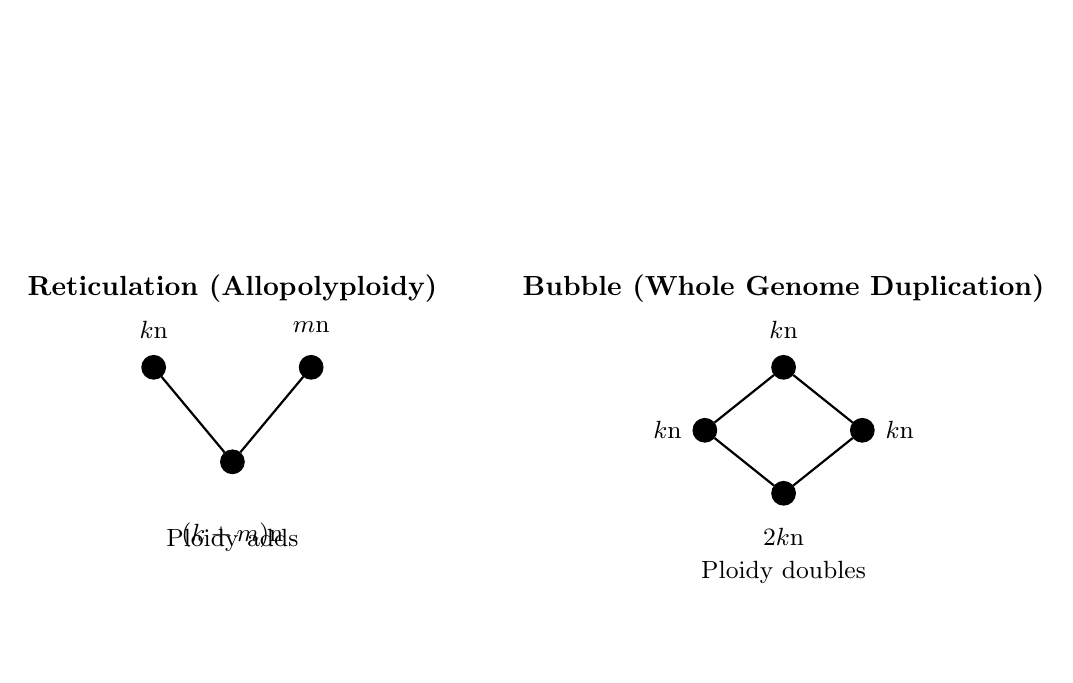
\begin{tikzpicture}[
        scale=1.0,
        every node/.style={circle, draw, fill=black, minimum size=3mm, inner sep=0pt},
        edge/.style={draw, thick},
    ]
    
    % === RETICULATION EXAMPLE ===
    \node[draw=none, fill=none] at (-4, 1) {\textbf{Reticulation (Allopolyploidy)}};
    
    \node (r1a) at (-5, 0) {};
    \node[draw=none, fill=none, above=0.1cm of r1a] {\small $k$n};
    
    \node (r1b) at (-3, 0) {};
    \node[draw=none, fill=none, above=0.1cm of r1b] {\small $m$n};
    
    \node (r1c) at (-4, -1.2) {};
    
    \draw[edge] (r1a) -- (r1c);
    \draw[edge] (r1b) -- (r1c);
    
    \node[draw=none, fill=none, below=0.1cm of r1c] {\small $(k+m)$n};
    
    \node[draw=none, fill=none] at (-4, -2.2) {\small Ploidy adds};
    
    % === BUBBLE EXAMPLE ===
    \node[draw=none, fill=none] at (3, 1) {\textbf{Bubble (Whole Genome Duplication)}};
    
    \node (b1) at (3, 0) {};
    \node[draw=none, fill=none, above=0.1cm of b1] {\small $k$n};
    
    \node (b2a) at (2, -0.8) {};
    \node (b2b) at (4, -0.8) {};
    
    \node (b3) at (3, -1.6) {};
    
    \draw[edge] (b1) -- (b2a);
    \draw[edge] (b1) -- (b2b);
    \draw[edge] (b2a) -- (b3);
    \draw[edge] (b2b) -- (b3);
    
    \node[draw=none, fill=none, left=0.1cm of b2a] {\small $k$n};
    \node[draw=none, fill=none, right=0.1cm of b2b] {\small $k$n};
    \node[draw=none, fill=none, below=0.1cm of b3] {\small $2k$n};
    
    \node[draw=none, fill=none] at (3, -2.6) {\small Ploidy doubles};
    
    \end{tikzpicture}
    \caption{The two ploidy-modifying structures in phylogenetic networks. \textbf{Left:} A reticulation (allopolyploidy) combines genetic material from two parent lineages, adding their ploidies. \textbf{Right:} A bubble (autopolyploidy/WGD) duplicates a single lineage's genome, doubling the ploidy.}
    \label{fig:ploidy-structures}
\end{figure}

\subsubsection{Network Definitions}

\begin{definition}[Valid Network]
A phylogenetic network $\Psi = (V, E)$ is \textit{valid} with respect to a ploidy assignment $\pi : \mathcal{X} \rightarrow \mathbb{Z}^+$ if for every leaf $x \in \mathcal{X}$, the ploidy function satisfies $p(x) = \pi(x)$.
\end{definition}

\begin{definition}[Binary Network]
A phylogenetic network is \textit{binary} if:
\begin{itemize}
    \item Every tree node (in-degree 1) has out-degree 2
    \item Every reticulation node (in-degree 2) has out-degree 1
    \item The root has in-degree 0 and out-degree 2
    \item Every leaf has in-degree 1 and out-degree 0
\end{itemize}
\end{definition}

\begin{definition}[Network Space]
Let $\mathcal{N}_\pi$ denote the set of all valid binary networks with respect to a fixed ploidy assignment $\pi$. This is the \textit{valid network space} that SRPP explores.
\end{definition}

\subsection{Constructing Arbitrary Ploidy Values}

A key observation enables our canonical network construction: any positive integer ploidy can be achieved through a combination of bubbles and reticulations from a ploidy-1 source.

\begin{lemma}[Ploidy Construction]\label{lem:ploidy-construction}
For any target ploidy $n \in \mathbb{Z}^+$, there exists a binary network structure that transforms ploidy 1 into ploidy $n$ using only bubbles and reticulations from ploidy-1 sources.
\end{lemma}

\begin{proof}
We construct the required ploidy using the following procedure:

\textbf{Step 1:} Let $k = \lfloor \log_2(n) \rfloor$. Construct a chain of $k$ bubbles. Starting from ploidy 1:
\[1 \xrightarrow{\text{bubble}} 2 \xrightarrow{\text{bubble}} 4 \xrightarrow{\text{bubble}} \cdots \xrightarrow{\text{bubble}} 2^k\]

\textbf{Step 2:} Let $r = n - 2^k$ be the remainder. Note that $0 \leq r < 2^k$ by definition of $k$.

\textbf{Step 3:} Add $r$ sequential reticulations, each from a ploidy-1 source. After the bubble chain produces ploidy $2^k$, each reticulation adds 1:
\begin{align*}
    \text{After 1st reticulation:} \quad & 2^k + 1 \\
    \text{After 2nd reticulation:} \quad & 2^k + 1 + 1 = 2^k + 2 \\
    & \vdots \\
    \text{After $r$th reticulation:} \quad & 2^k + r = n
\end{align*}

Each reticulation node has in-degree 2 (one edge from the chain above, one edge from a ploidy-1 source), maintaining binary structure.
\end{proof}

\begin{figure}[H]
    \centering
    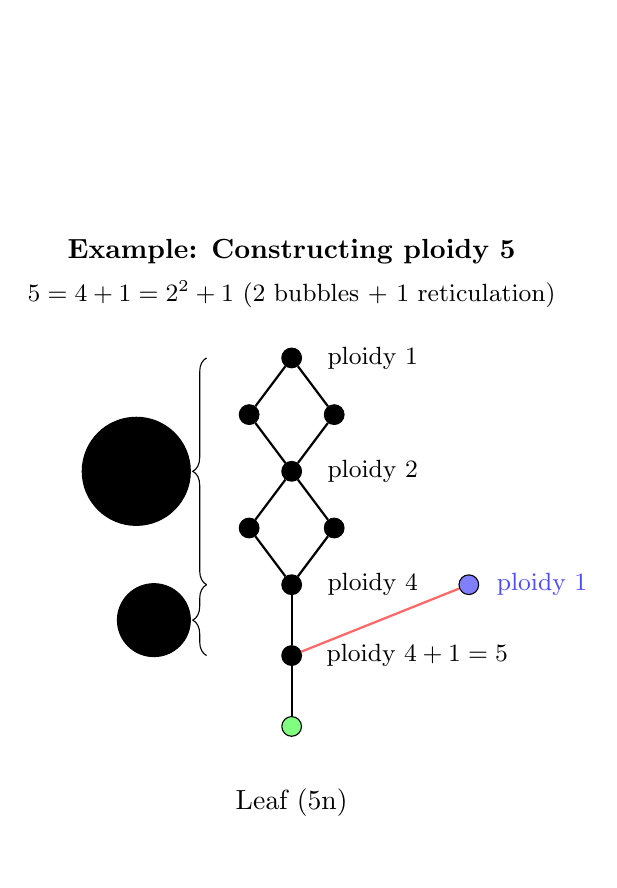
\begin{tikzpicture}[
        scale=0.9,
        every node/.style={circle, draw, fill=black, minimum size=2.5mm, inner sep=0pt},
        edge/.style={draw, thick},
        spine/.style={draw, thick, blue!60},
        retic/.style={draw, thick, red!60},
    ]
    
    % === Example: Building ploidy 5 ===
    \node[draw=none, fill=none] at (0, 1) {\textbf{Example: Constructing ploidy 5}};
    \node[draw=none, fill=none] at (0, 0.4) {\small $5 = 4 + 1 = 2^2 + 1$ (2 bubbles + 1 reticulation)};
    
    % Starting node
    \node (start) at (0, -0.5) {};
    \node[draw=none, fill=none, right=0.3cm of start] {\small ploidy 1};
    
    % Bubble 1
    \node (b1L) at (-0.6, -1.3) {};
    \node (b1R) at (0.6, -1.3) {};
    \draw[edge] (start) -- (b1L);
    \draw[edge] (start) -- (b1R);
    
    \node (b1out) at (0, -2.1) {};
    \draw[edge] (b1L) -- (b1out);
    \draw[edge] (b1R) -- (b1out);
    \node[draw=none, fill=none, right=0.3cm of b1out] {\small ploidy 2};
    
    % Bubble 2
    \node (b2L) at (-0.6, -2.9) {};
    \node (b2R) at (0.6, -2.9) {};
    \draw[edge] (b1out) -- (b2L);
    \draw[edge] (b1out) -- (b2R);
    
    \node (b2out) at (0, -3.7) {};
    \draw[edge] (b2L) -- (b2out);
    \draw[edge] (b2R) -- (b2out);
    \node[draw=none, fill=none, right=0.3cm of b2out] {\small ploidy 4};
    
    % Reticulation from spine
    \node[fill=blue!50] (spine1) at (2.5, -3.7) {};
    \node[draw=none, fill=none, right=0.2cm of spine1] {\small \textcolor{blue!70}{ploidy 1}};
    
    \node (retic1) at (0, -4.7) {};
    \draw[edge] (b2out) -- (retic1);
    \draw[retic] (spine1) -- (retic1);
    \node[draw=none, fill=none, right=0.3cm of retic1] {\small ploidy $4+1=5$};
    
    % Leaf
    \node[fill=green!50] (leaf) at (0, -5.7) {};
    \draw[edge] (retic1) -- (leaf);
    \node[draw=none, fill=none, below=0.1cm of leaf] {Leaf (5n)};
    
    % Annotations
    \draw[decorate, decoration={brace, amplitude=5pt, mirror}] (-1.2, -0.5) -- (-1.2, -3.7) node[midway, left=0.2cm] {\small 2 bubbles};
    \draw[decorate, decoration={brace, amplitude=5pt, mirror}] (-1.2, -3.7) -- (-1.2, -4.7) node[midway, left=0.2cm] {\small 1 retic};
    
    \end{tikzpicture}
    \caption{Constructing ploidy 5 from ploidy 1. Two bubbles produce $2^2 = 4$, then one reticulation from a ploidy-1 source adds 1, yielding $4 + 1 = 5$.}
    \label{fig:ploidy-construction}
\end{figure}

\begin{remark}[Efficiency of Construction]
To achieve ploidy $n$, we need at most $\lfloor \log_2(n) \rfloor$ bubbles and at most $n - 2^{\lfloor \log_2(n) \rfloor} < n/2$ reticulations. The total number of operations is $O(\log n + n/2) = O(n)$.
\end{remark}

\subsection{Existence of Canonical Networks}

We now establish that for any ploidy assignment, a canonical network structure exists.

\begin{definition}[Ploidy Spine]
A \textit{ploidy spine} is a linear chain of nodes $S_1, S_2, \ldots, S_\ell$ attached to the root such that each spine node has ploidy 1. The spine is constructed as a sequence of tree nodes branching off from the main network, with each $S_i$ having out-degree 2: one edge continues to $S_{i+1}$ (or terminates), and one edge is available as a reticulation source.
\end{definition}

\begin{algorithm}[H]
\caption{ConstructCanonicalNetwork}\label{alg:canonical}
\textbf{Input:} Ploidy assignment $\pi: \mathcal{X} \rightarrow \mathbb{Z}^+$ where $\mathcal{X} = \{x_1, \ldots, x_n\}$

\textbf{Output:} Valid binary network $\Psi^*$ satisfying $\pi$

\begin{algorithmic}[1]
    \Procedure{ConstructCanonical}{$\pi$}
        \State Create root node $r$
        
        \State \textit{// Calculate spine length needed}
        \State $R_{total} \gets \sum_{x \in \mathcal{X}} \left( \pi(x) - 2^{\lfloor \log_2(\pi(x)) \rfloor} \right)$ \Comment{Total reticulations needed}
        \State Create ploidy spine of length $R_{total}$ as right subtree of $r$
        
        \State \textit{// Initialize structure for leaves}
        \State Initialize left subtree of $r$ as caterpillar backbone
        \State $spine\_index \gets 1$
        
        \For{each leaf $x_i \in \mathcal{X}$}
            \State $k \gets \lfloor \log_2(\pi(x_i)) \rfloor$ \Comment{Number of bubbles}
            \State $r_i \gets \pi(x_i) - 2^k$ \Comment{Number of reticulations}
            \State 
            \State \textit{// Build bubble chain}
            \State Create chain of $k$ bubbles
            \State Attach chain to next position in caterpillar backbone
            \State
            \State \textit{// Add sequential reticulations for remainder}
            \State $current \gets$ bottom of bubble chain
            \For{$j = 1$ to $r_i$}
                \State Create new reticulation node $v$
                \State Connect $current \to v$
                \State Connect $S_{spine\_index} \to v$ \Comment{From ploidy-1 spine}
                \State $current \gets v$
                \State $spine\_index \gets spine\_index + 1$
            \EndFor
            \State
            \State Attach leaf $x_i$ below $current$
        \EndFor
        
        \State \Return $\Psi^*$
    \EndProcedure
\end{algorithmic}
\end{algorithm}

\begin{lemma}[Canonical Network Existence]\label{lem:existence}
For any ploidy assignment $\pi: \mathcal{X} \rightarrow \mathbb{Z}^+$, there exists a valid binary network $\Psi^* \in \mathcal{N}_\pi$.
\end{lemma}

\begin{proof}
We show that Algorithm~\ref{alg:canonical} produces a valid binary network.

\textbf{Correctness of ploidy:} For each leaf $x_i$ with target ploidy $\pi(x_i)$:
\begin{itemize}
    \item Let $k = \lfloor \log_2(\pi(x_i)) \rfloor$. The chain of $k$ bubbles produces ploidy $2^k$.
    
    \item Let $r_i = \pi(x_i) - 2^k$. We add $r_i$ sequential reticulations, each from a spine node with ploidy 1.
    
    \item At each reticulation node, the incoming ploidy from above is added to 1 from the spine:
    \begin{align*}
        \text{After bubble chain:} \quad & 2^k \\
        \text{After 1st reticulation:} \quad & 2^k + 1 \\
        \text{After 2nd reticulation:} \quad & (2^k + 1) + 1 = 2^k + 2 \\
        & \vdots \\
        \text{After $r_i$th reticulation:} \quad & 2^k + r_i = \pi(x_i)
    \end{align*}
\end{itemize}

\textbf{Binary constraints:} 
\begin{itemize}
    \item \textit{Bubbles:} The top node has out-degree 2; the bottom node has in-degree 2 and out-degree 1 (or 2 if another bubble follows).
    
    \item \textit{Reticulation nodes:} Each has in-degree 2 (one from chain above, one from spine) and out-degree 1.
    
    \item \textit{Spine nodes:} Each has out-degree 2 (one continuing spine, one to reticulation).
    
    \item \textit{Caterpillar backbone:} Standard binary tree structure.
\end{itemize}

\textbf{Sufficient spine length:} The total reticulations needed is:
\[R_{total} = \sum_{x_i \in \mathcal{X}} \left( \pi(x_i) - 2^{\lfloor \log_2(\pi(x_i)) \rfloor} \right)\]
The spine provides exactly $R_{total}$ nodes, each used once.

Therefore, $\Psi^*$ is a valid binary network in $\mathcal{N}_\pi$.
\end{proof}

\begin{figure}[H]
    \centering
    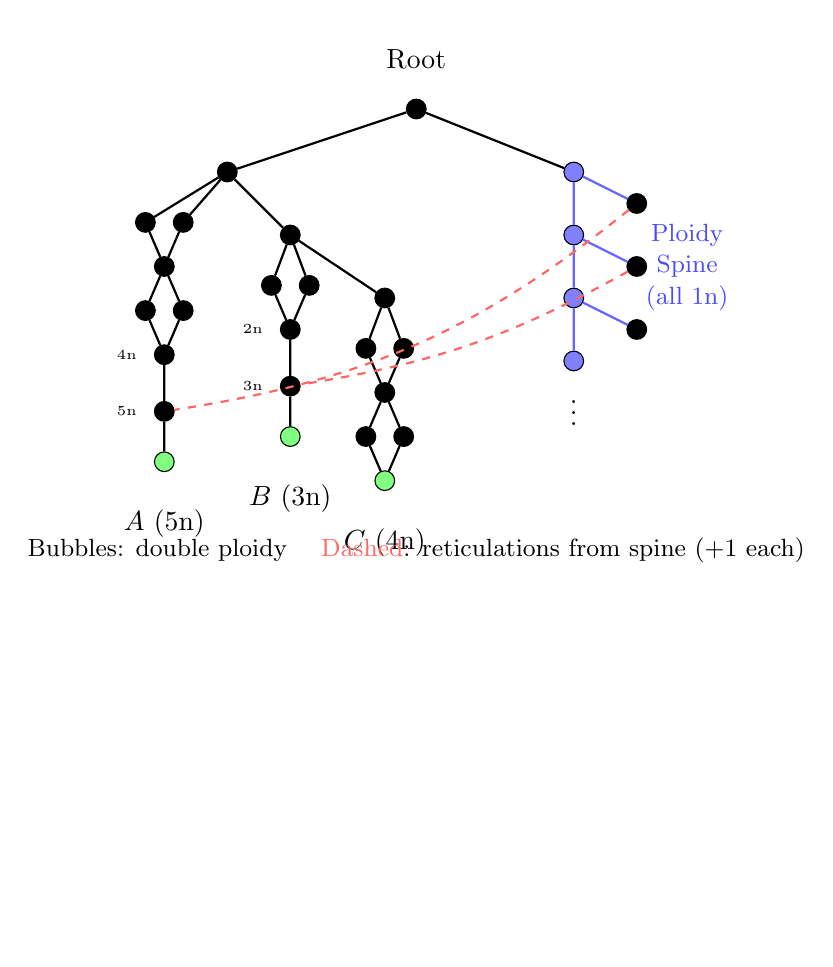
\begin{tikzpicture}[
        scale=0.8,
        every node/.style={circle, draw, fill=black, minimum size=2.5mm, inner sep=0pt},
        edge/.style={draw, thick},
        spine/.style={draw, thick, blue!60},
        retic/.style={draw, thick, red!60, dashed},
    ]
    
    % Root
    \node[fill=black] (root) at (0, 0) {};
    \node[draw=none, fill=none, above=0.1cm of root] {Root};
    
    % === LEFT SIDE: Caterpillar with bubble chains ===
    \node (L1) at (-3, -1) {};
    \draw[edge] (root) -- (L1);
    
    % --- A's structure (ploidy 5 = 4 + 1) ---
    % Bubble 1
    \node (A1a) at (-4.3, -1.8) {};
    \node (A1b) at (-3.7, -1.8) {};
    \draw[edge] (L1) -- (A1a);
    \draw[edge] (L1) -- (A1b);
    
    \node (A2) at (-4, -2.5) {};
    \draw[edge] (A1a) -- (A2);
    \draw[edge] (A1b) -- (A2);
    
    % Bubble 2
    \node (A3a) at (-4.3, -3.2) {};
    \node (A3b) at (-3.7, -3.2) {};
    \draw[edge] (A2) -- (A3a);
    \draw[edge] (A2) -- (A3b);
    
    \node (A4) at (-4, -3.9) {};
    \draw[edge] (A3a) -- (A4);
    \draw[edge] (A3b) -- (A4);
    \node[draw=none, fill=none, left=0.2cm of A4] {\tiny 4n};
    
    % Reticulation for +1
    \node (A5) at (-4, -4.8) {};
    \draw[edge] (A4) -- (A5);
    \node[draw=none, fill=none, left=0.2cm of A5] {\tiny 5n};
    
    \node[fill=green!50] (A) at (-4, -5.6) {};
    \draw[edge] (A5) -- (A);
    \node[draw=none, fill=none, below=0.1cm of A] {$A$ (5n)};
    
    % --- Continue caterpillar ---
    \node (cat1) at (-2, -2) {};
    \draw[edge] (L1) -- (cat1);
    
    % --- B's structure (ploidy 3 = 2 + 1) ---
    % Bubble 1
    \node (B1a) at (-2.3, -2.8) {};
    \node (B1b) at (-1.7, -2.8) {};
    \draw[edge] (cat1) -- (B1a);
    \draw[edge] (cat1) -- (B1b);
    
    \node (B2) at (-2, -3.5) {};
    \draw[edge] (B1a) -- (B2);
    \draw[edge] (B1b) -- (B2);
    \node[draw=none, fill=none, left=0.2cm of B2] {\tiny 2n};
    
    % Reticulation for +1
    \node (B3) at (-2, -4.4) {};
    \draw[edge] (B2) -- (B3);
    \node[draw=none, fill=none, left=0.2cm of B3] {\tiny 3n};
    
    \node[fill=green!50] (B) at (-2, -5.2) {};
    \draw[edge] (B3) -- (B);
    \node[draw=none, fill=none, below=0.1cm of B] {$B$ (3n)};
    
    % --- Continue caterpillar ---
    \node (cat2) at (-0.5, -3) {};
    \draw[edge] (cat1) -- (cat2);
    
    % --- C's structure (ploidy 4 = 4 + 0, no reticulations) ---
    % Bubble 1
    \node (C1a) at (-0.8, -3.8) {};
    \node (C1b) at (-0.2, -3.8) {};
    \draw[edge] (cat2) -- (C1a);
    \draw[edge] (cat2) -- (C1b);
    
    \node (C2) at (-0.5, -4.5) {};
    \draw[edge] (C1a) -- (C2);
    \draw[edge] (C1b) -- (C2);
    
    % Bubble 2
    \node (C3a) at (-0.8, -5.2) {};
    \node (C3b) at (-0.2, -5.2) {};
    \draw[edge] (C2) -- (C3a);
    \draw[edge] (C2) -- (C3b);
    
    \node[fill=green!50] (C) at (-0.5, -5.9) {};
    \draw[edge] (C3a) -- (C);
    \draw[edge] (C3b) -- (C);
    \node[draw=none, fill=none, below=0.1cm of C] {$C$ (4n)};
    
    % === RIGHT SIDE: Ploidy spine ===
    \node[fill=blue!50] (S1) at (2.5, -1) {};
    \draw[edge] (root) -- (S1);
    
    \node[fill=blue!50] (S2) at (2.5, -2) {};
    \node (S1out) at (3.5, -1.5) {};
    \draw[spine] (S1) -- (S2);
    \draw[spine] (S1) -- (S1out);
    
    \node[fill=blue!50] (S3) at (2.5, -3) {};
    \node (S2out) at (3.5, -2.5) {};
    \draw[spine] (S2) -- (S3);
    \draw[spine] (S2) -- (S2out);
    
    \node[fill=blue!50] (S4) at (2.5, -4) {};
    \node (S3out) at (3.5, -3.5) {};
    \draw[spine] (S3) -- (S4);
    \draw[spine] (S3) -- (S3out);
    
    \node[draw=none, fill=none] at (2.5, -4.7) {$\vdots$};
    
    % Spine labels
    \node[draw=none, fill=none] at (4.3, -2) {\small \textcolor{blue!70}{Ploidy}};
    \node[draw=none, fill=none] at (4.3, -2.5) {\small \textcolor{blue!70}{Spine}};
    \node[draw=none, fill=none] at (4.3, -3) {\small \textcolor{blue!70}{(all 1n)}};
    
    % === RETICULATION EDGES ===
    \draw[retic] (S1out) to[bend left=15] (A5);
    \draw[retic] (S2out) to[bend left=10] (B3);
    
    % Legend
    \node[draw=none, fill=none] at (0, -7) {\small Bubbles: double ploidy \quad \textcolor{red!60}{Dashed}: reticulations from spine (+1 each)};
    
    \end{tikzpicture}
    
    \caption{Canonical network $\Psi^*$ for $\pi(A) = 5$, $\pi(B) = 3$, $\pi(C) = 4$. Left: caterpillar backbone with bubble chains. Right: ploidy spine (blue, all nodes have ploidy 1). Red dashed edges are reticulations that each add 1 to the ploidy. Leaf $A$: 2 bubbles ($1 \to 2 \to 4$) + 1 reticulation ($4+1=5$). Leaf $B$: 1 bubble ($1 \to 2$) + 1 reticulation ($2+1=3$). Leaf $C$: 2 bubbles ($1 \to 2 \to 4$), no reticulations needed.}
    \label{fig:canonical}
\end{figure}

\subsection{Reachability}

With the existence of canonical networks established, we now prove that SRPP can transform any valid network into any other valid network.

\begin{lemma}\label{lem:to-canonical}
For any valid binary network $\Psi \in \mathcal{N}_\pi$, there exists a sequence of SRPP moves that transforms $\Psi$ into a canonical network $\Psi^*$.
\end{lemma}

\begin{proof}
We prove this by strong induction on $n = |\mathcal{X}|$, the number of leaves.

\textbf{Base case} ($n = 1$): With a single leaf $x$, any valid binary network delivers ploidy $\pi(x)$ to $x$ through some combination of bubbles and reticulations. Apply SRPP to $x$: disconnect $\Psi_x$ and reattach it with the canonical structure (appropriate bubbles followed by reticulations from a spine). This requires at most 2 SRPP moves.

\textbf{Inductive step}: Assume the claim holds for all networks with fewer than $n$ leaves. Let $\Psi \in \mathcal{N}_\pi$ have $n$ leaves.

\textit{Step 1:} Select any leaf $x_1 \in \mathcal{X}$. Apply SRPP to disconnect sub-network $\Psi_{x_1}$ and reattach $x_1$ in canonical configuration:
\begin{itemize}
    \item Position in leftmost caterpillar slot
    \item $k_1 = \lfloor \log_2(\pi(x_1)) \rfloor$ bubbles
    \item $r_1 = \pi(x_1) - 2^{k_1}$ sequential reticulations from spine
\end{itemize}
This requires at most 2 SRPP moves.

\textit{Step 2:} The remaining sub-network has $(n-1)$ leaves. By the inductive hypothesis, it can be transformed to canonical form.

\textit{Step 3:} Repositioning remaining leaves does not affect $x_1$ (SRPP preserves ploidy outside the operated sub-network).

By induction, any network reaches $\Psi^*$ in at most $2n$ SRPP moves.
\end{proof}

\begin{lemma}\label{lem:from-canonical}
For any valid binary network $\Psi \in \mathcal{N}_\pi$, there exists a sequence of SRPP moves that transforms a canonical network $\Psi^*$ into $\Psi$.
\end{lemma}

\begin{proof}
The proof mirrors Lemma~\ref{lem:to-canonical} by strong induction on $n = |\mathcal{X}|$.

\textbf{Base case} ($n = 1$): Analogous to Lemma~\ref{lem:to-canonical}.

\textbf{Inductive step}: Let $\Psi$ be the target network with $n$ leaves.

\textit{Step 1:} Identify leaf $x_1$ and its configuration in target $\Psi$.

\textit{Step 2:} In $\Psi^*$, apply SRPP to $x_1$: disconnect from canonical position and reattach according to $\Psi$'s configuration. At most 2 SRPP moves.

\textit{Step 3:} Transform remaining $(n-1)$ leaves by inductive hypothesis.

By induction, $\Psi^*$ reaches any network in at most $2n$ SRPP moves.
\end{proof}

\begin{theorem}[Reachability]\label{thm:reachability}
For any two valid binary networks $\Psi_1, \Psi_2 \in \mathcal{N}_\pi$, there exists a sequence of SRPP moves that transforms $\Psi_1$ into $\Psi_2$. 
\end{theorem}

\begin{proof}
By Lemma~\ref{lem:to-canonical}, $\Psi_1 \to \Psi^*$. By Lemma~\ref{lem:from-canonical}, $\Psi^* \to \Psi_2$. Composition yields $\Psi_1 \to \Psi_2$.
\end{proof}

\subsection{Invertibility}

\begin{theorem}[Invertibility]\label{thm:invertibility}
Every SRPP move is invertible: for any SRPP move $m: \Psi \to \Psi'$, there exists an SRPP move $m^{-1}: \Psi' \to \Psi$.
\end{theorem}

\begin{proof}
Let $m$ operate on node $n$ in network $\Psi$:
\begin{enumerate}
    \item \textbf{Disconnection:} $m$ removes edges $E_{old}$ connecting $\Psi_n$ to its MSWLEs.
    \item \textbf{Reattachment:} $m$ creates edges $E_{new}$ to restore ploidy $p(n)$.
\end{enumerate}

The inverse $m^{-1}$ on $\Psi'$:
\begin{enumerate}
    \item Select same node $n$ (persists as root of $\Psi_n$ in $\Psi'$).
    \item \textbf{Disconnection:} Remove edges $E_{new}$.
    \item \textbf{Reattachment:} Recreate edges to original attachment points of $E_{old}$.
\end{enumerate}

This is valid because:
\begin{itemize}
    \item Node $n$ remains non-root in $\Psi'$
    \item Original attachment points persist (external to $\Psi_n$)
    \item Original ploidy $p(n)$ is achievable via $E_{old}$
\end{itemize}

Thus $m^{-1}(m(\Psi)) = \Psi$.
\end{proof}

\begin{corollary}
SRPP defines a symmetric adjacency relation on $\mathcal{N}_\pi$.
\end{corollary}

\subsection{Network Search Space Diameter}

\begin{theorem}[Diameter Bound]\label{thm:diameter}
The diameter of $\mathcal{N}_\pi$ under SRPP moves is at most $4|\mathcal{X}|$.
\end{theorem}

\begin{proof}
For any $\Psi_1, \Psi_2 \in \mathcal{N}_\pi$:
\[
d(\Psi_1, \Psi_2) \leq d(\Psi_1, \Psi^*) + d(\Psi^*, \Psi_2) \leq 2|\mathcal{X}| + 2|\mathcal{X}| = 4|\mathcal{X}|
\]
\end{proof}

\begin{remark}
The bound $4|\mathcal{X}|$ is not tight:
\begin{enumerate}
    \item Similar networks may transform directly without visiting $\Psi^*$
    \item Single SRPP moves can adjust multiple leaves sharing a sub-network
    \item The inductive construction is pessimistic
\end{enumerate}
\end{remark}

\begin{corollary}[Ergodicity]
A random walk on $\mathcal{N}_\pi$ using SRPP is ergodic. Combined with invertibility, MCMC methods using SRPP converge to the correct stationary distribution.
\end{corollary}


\section{Theoretical Computational Savings: MP-Allop-2.0 vs InferNetwork-MP-Allop}

\paragraph{\color{bluem}MP-Allop-2.0} Since each move is guaranteed to propose a valid network, it is easier to predict the cost/speed of moving around the network space, and thus convergence times should be more consistent. An in-depth analysis of the pseudocode algorithms in section 6 is included (new section + link to it), and it turns out that the cost of the move is O(V + E), coming from the requirement that each node and edge needs to be checked for its ploidy value (line 6 algorithm 1). 

\paragraph{\color{bluem} InferNetwork-MP-Allop} Each move is randomly selected from a set of 6 network moves:
\begin{enumerate}
    \item AddReticulation
    \item RemoveReticulation
    \item RelocateReticulationSource
    \item RelocateReticulationDestination
    \item FlipReticulation
    \item RelocateReticulation
\end{enumerate}

Each of these moves does not guarantee that a network will 1) have the correct ploidy at the tips 2) not contain a cycle. Or, work has to be done to avoid the creation of a cycle, and doing that requires knowledge of the edges that would avoid the creation of a cycle. That is \textit{exactly} as expensive as doing SRPP in the first place.

Therefore, the amount of extra work that InferNetwork-MP-Allop has to do depends directly on the proportion of moves that get discarded and the convergence timing for each move set.

It should also be noted that moves 1 and 2 are guaranteed to introduce an invalid network given a valid network. If the ploidy at the tips is what it should be, then adding or removing a reticulation is guaranteed to leave the network in a state where there is too much or not enough ploidy at the tips. Since moves are randomly chosen, that is 1/3 of the time that a move has to be discarded, at a bare minimum (presuming nothing has been done about this important technicality).

At this point, it should be clear that introducing a bit of upfront work to maintain the validity of proposed networks has only positive upside, which is closely proportional to the amount of invalid networks that InferNetwork-MP-Allop proposes in its kernel.


\section{Data and Results}

Here in this paper, we use the same simulated data (Scenarios D, E, F, J) as described in the section "Simulations" of \cite{YanMP} :

"We used the AlloppDT simulator (Jones 2012) and parameter settings of Jones et al. (2013) and Jones (2017) to simulate a collection of data sets. The data were generated under four different evolutionary scenarios with 1, 2, 3 and 3 reticulations (Fig. 3), where for each scenario the mutation rate, the number of individuals per species, and the number of genes were varied. In addition, we increased the number of genes to 100 to emulate the kinds of data sets enabled by next-generation sequencing. In total, there were 116 model conditions, each with 10 replicate data sets (Table 1). Since the gene tree-based inference methods considered in this study require rooted gene trees, an outgroup species was added for the purpose of rooting the estimated gene trees Table 1 and was excluded in the species phylogeny reconstruction. It would be possible for molecular clock methods to root the gene trees by finding the tree with the best ultrametric fit, but this may be unreliable when the strict molecular clock assumption is violated."


\subsection{\color{bluem}Accuracy and Species Network Error}

\subsection{\color{bluem}Runtime and Performance Comparisons}


\section{Algorithms} \label{Algs}
In this section are pseudocode algorithms for the SRPP move and other related implementation details. For the following algorithms, let P(n) or P(e) denote the current node or edge ploidy in the network-- these values are gathered by map lookups after a CalculatePloidy call. This is for brevity.

\begin{algorithm}[H]
\caption{CalculatePloidy}\label{euclid}

\textbf{Inputs:} 
\begin{enumerate}
    \item Directed Acyclic Graph (DAG) G = (V, E)
    
\end{enumerate}
\textbf{Output:}
\begin{enumerate}
    \item 2 mappings, one from V $\rightarrow \mathbf{N}$ and one from E $\rightarrow \mathbf{N}$, mapping nodes and edges to ploidy values.
\end{enumerate}

  \begin{algorithmic}[1]
    \Procedure{CalculatePloidy}{$G$}
        \State node\_ploidy $\gets$ empty mapping
        \State edge\_ploidy $\gets$ empty mapping
        \State visited $\gets$ empty set
        
        \State bfs\_start $\gets$ G.root
        \State Q $\gets$ empty queue
        \State Q.push(bfs\_start)
        \State node\_ploidy[bfs\_start] $\gets$ 1 \Comment{Set other nodes to 0}
        \While{Q is not empty}
            \State cur $\gets$ Q.pop()
            \If{cur $\notin$ visited}
                \For{parent in cur.parents} \Comment{Node rule}
                    \State node\_ploidy[cur] $\gets$ node\_ploidy[cur] + node\_ploidy[par] 
                \EndFor
                \For{child in cur.children} \Comment{Edge rule}
                    \State edge\_ploidy[(cur, child)] $\gets$ node\_ploidy[cur]
                    \State Q.push(child)
                \EndFor
            \EndIf
            \State add cur to visited set
        \EndWhile
    \State \Return node\_ploidy, edge\_ploidy
    \EndProcedure
  \end{algorithmic}


\end{algorithm}



\begin{algorithm}[H]
\caption{Sub-Network Redirect and Preserve Ploidy}\label{euclid}

\textbf{Inputs:} 
\begin{enumerate}
    \item Directed Acyclic Graph (DAG) G = (V, E)
    
\end{enumerate}
\textbf{Output:}
\begin{enumerate}
    \item A different DAG, G' = (V', E')
\end{enumerate}

  \begin{algorithmic}[1]
    \Procedure{SRPP}{$G$}
    
        \State node $\gets$ select random node in \(V - \{root\}\)
        \While{node.sibling.is\_leaf() $=$ True $\land$ node.parents $=$ \{root\}}
            \State node $\gets$ select random node in \(V - \{root\}\) 
        \EndWhile

        \State target $\gets$ P(node)
        \State \textit{DisconnectMSWLE(G, node)}
        \State \textit{Reattach(G, node, target)}

        \Return G
        
    \EndProcedure
  \end{algorithmic}


\end{algorithm}


\begin{algorithm}[H]
\caption{DisconnectMSWLE}\label{euclid}

\textbf{Inputs:} 
\begin{enumerate}
    \item Directed Acyclic Graph (DAG) $\Psi = (V, E)$
    \item Node $n \in V$, $n$ is not the root of $\Psi$
\end{enumerate}

  \begin{algorithmic}[1]
    \Procedure{DisconnectMSWLE}{$\Psi, n$}
        \State $e$ $\gets$ random in-edge of $n$
        \State $Q \gets$ empty queue
        \State $prev \gets$ $n$
        \State $Q$.push($e_{src}$) \Comment{$n$ is $e_{dest}$}
        
        \While{$Q \neq \varnothing$}
            \State $cur \gets Q$.pop()
            \State Delete edge $(cur,$ $prev)$ from $E$
            \If{$\mathcal{L}_{cur} \neq \mathcal{L}_n$} \Comment{Found MSWLE}
                \State \textbf{Continue}
            \EndIf
            \For{parent $p$ of $cur$}
                \State $Q$.push($p$)
            \EndFor
            \State $prev \gets$ $cur$
            \State Delete node $cur$ from $V$
        \EndWhile
    \State 
    \EndProcedure
  \end{algorithmic}


\end{algorithm}



\begin{algorithm}[H]
\caption{Reattach}\label{euclid}

\textbf{Inputs:} 
\begin{enumerate}
    \item Directed Acyclic Graph (DAG) G = (V, E)
    \item node $n \in V$
    \item target (goal ploidy for n)
\end{enumerate}

  \begin{algorithmic}[1]
    \Procedure{Reattach}{$G$, $n$, $target$}

    \State valid\_srcs $\gets$ \{n\}
    
    \While{P(n) $\neq$ target}
        \State cur\_src $\gets$ random node/edge from valid\_srcs
        \State valid\_edges $\gets$ \( \{e \in E | P(e) \leq target - P(n)\}\)
        \State e $\gets$ random edge in valid\_edges
        
        \If{cur\_src is a node} \Comment{Initial case}
            \State v $\gets$ new edge from cur\_src to e
            \State valid\_srcs $\gets$ valid\_srcs - {cur\_src}
        \EndIf
        \If{cur\_src is an edge} \Comment{Every iteration thereafter}
            \State new\_src $\gets$ A new node 
            \State insert new\_src into cur\_src
            \State v $\gets$ new edge from new\_src to e
        \EndIf
        \State valid\_srcs $\gets$ valid\_srcs $\cup$ v
        \If{e $\in$ valid\_srcs}
            \Comment{edge e was split into $e_1$ and $e_2$}
            \State valid\_srcs $\gets$ valid\_srcs - $\{e\} \cup \{e_1, e_2\}$ 
        \EndIf
        
    \EndWhile
        
    \EndProcedure
  \end{algorithmic}


\end{algorithm}
\bibliographystyle{abbrv}
\bibliography{refs}
\end{document}
